\chapter{Background}

\section{Norway and Sea level Extremes in the Present Day}
The Norwegian coastlines including its many small islands has been estimated to be 83,281 km \cite{aunan_strong_2008}. Considering the entire kingdom of Norway including Svalbard is only 384 486 km² \cite{engelien_area_2022}, it would be reasonable to consider Norway as dominated by its relationship with the sea. This can be further supported by the presence of all its major cities along the coasts and that by January 2022, 31.6 percent of Norway's coastal zone has been influenced by buildings, railways, roads and agriculture \cite{engebakken_construction_2022}. Which combined with only 68.4 percent of the Norwegian coastline being deemed accessible \cite{engebakken_construction_2022}, displays the large amounts of infrastructure and population which reside along the Norwegian coastline. Norwegian weather is predicted to get more extreme \cite{rod_integrated_2012}. in line with global trends coastal flooding due to extreme weather and sea level rise will increase \cite{hoffken_effects_2020}. 
\paragraph{}

Due to changing climate and settlement patterns in Norway there is a increase in the threat of natural hazards from the sea, which require more attention spent on regional vulnerability and the resilience of places \cite{opach_seeking_2020} and \cite{rod_three_2015} . Quantitative community resilience measurement approaches have been tried, but there is several limiting factors in their results and most importantly they rarely offer policy makers the strategies they need \cite{opach_seeking_2020} and \cite{gerkensmeier_governing_2018}. There is important information which can be gained from vulnerability indices including understanding of social vulnerability, but questions remain about how social vulnerability can be improved upon, to build resilience. 


\section{Introduction to Research Area}

Trondheim is situated in a protected location, deep within Trondheimsfjord, which protects it from the North Sea. This protected location combined with the geological setting means that the assumption could be that Trondheim is not a risk from sea level extremes. This is further exaggerated by the understanding that Norwegian land is rising due to glacial melt. However, isostatic uplift is an incredibly varied process across the country and the basic model that the majority of the population has about sea level rise and land rise, may be creating a false confidence.  The maximum observed sea level extreme in Trondheim is 2.06m (NN2000), recorded in 1971 \cite{tides_high_2022}. Trondheim municipality plans indicate the city should be prepared for 4.87m by 2100. 

\begin{figure}[h!]
    \centering
    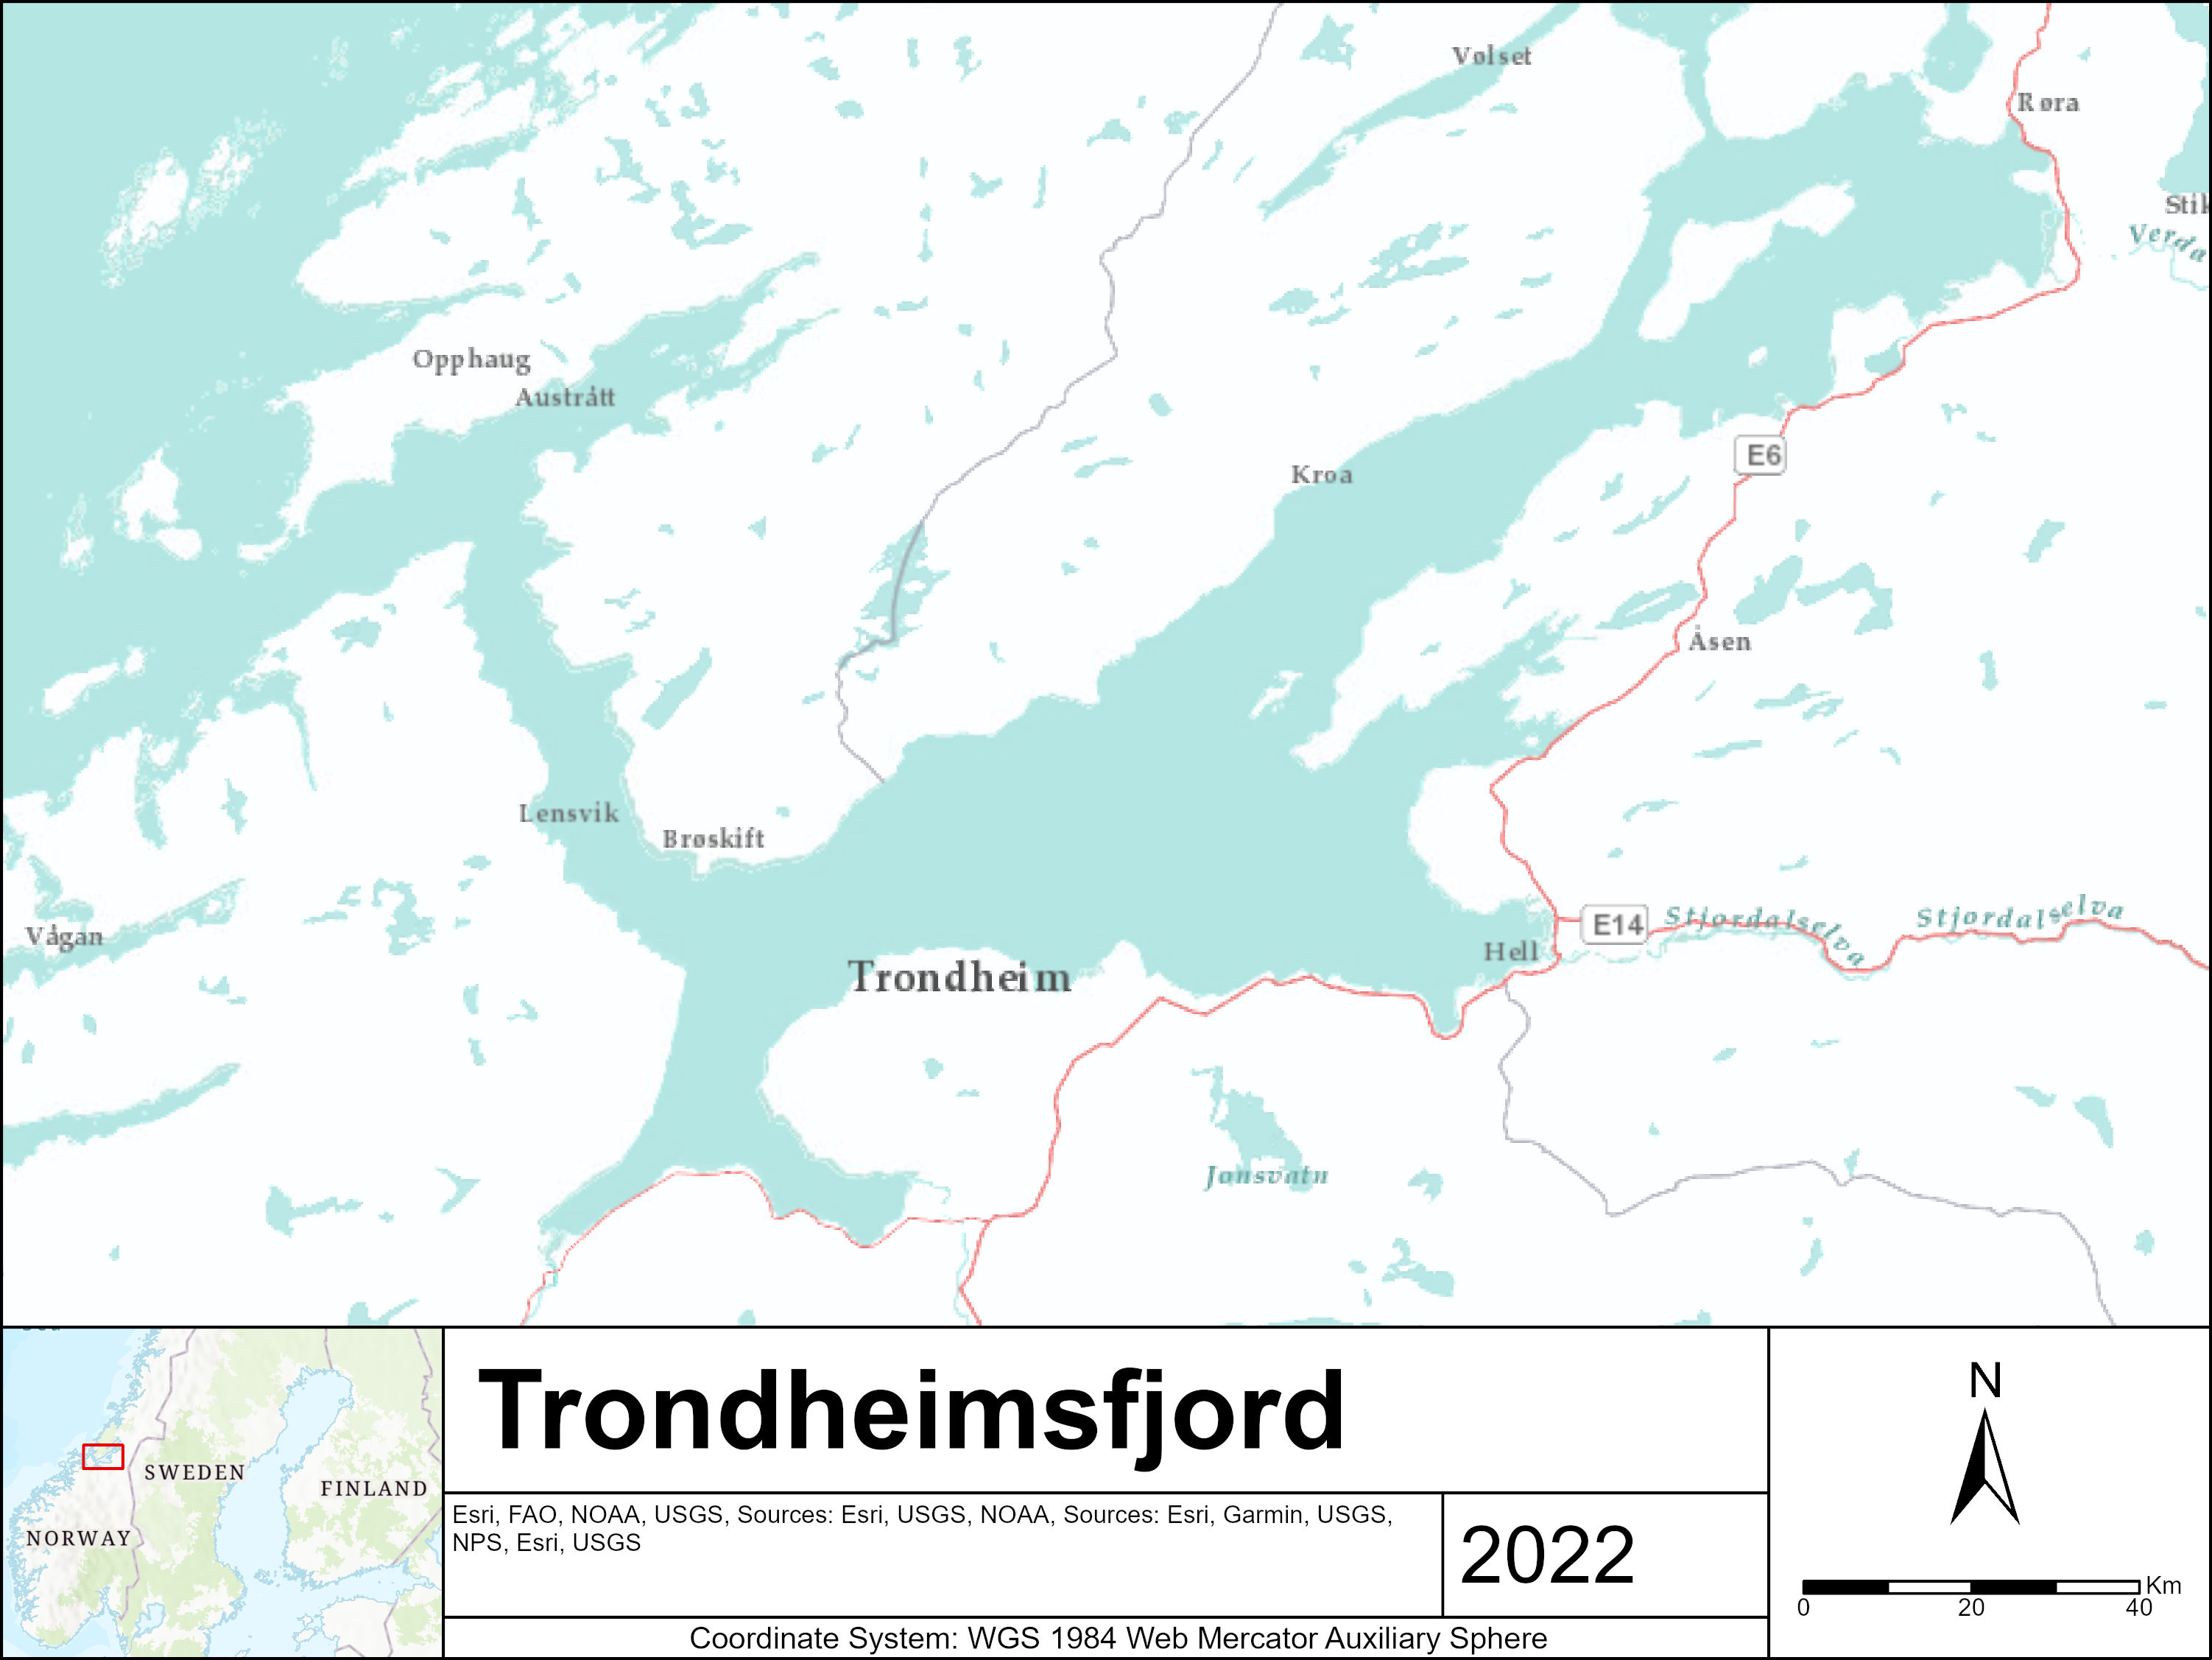
\includegraphics[width=1.0\textwidth]{fig/Trondheimsfjord.png}
    \caption{The location of Trondheim - The city is situated in Trondheimsfjord, which provides protection to the North Sea. Figure created using ArcGIS Pro}
    \label{fig:research area Trondheim}
\end{figure}



\section{Research Sites}
Four sites which are situated on Trondheim's coast were chosen to represent the resilience for the city. These locations were chosen for their high daily population throughput and large amounts of infrastructure. The physical vulnerability to sea level extremes is diverse for these sites as can be seen in figure** below and is further outlined in table** below. 
\paragraph{}

\begin{figure} [h]
    \centering
    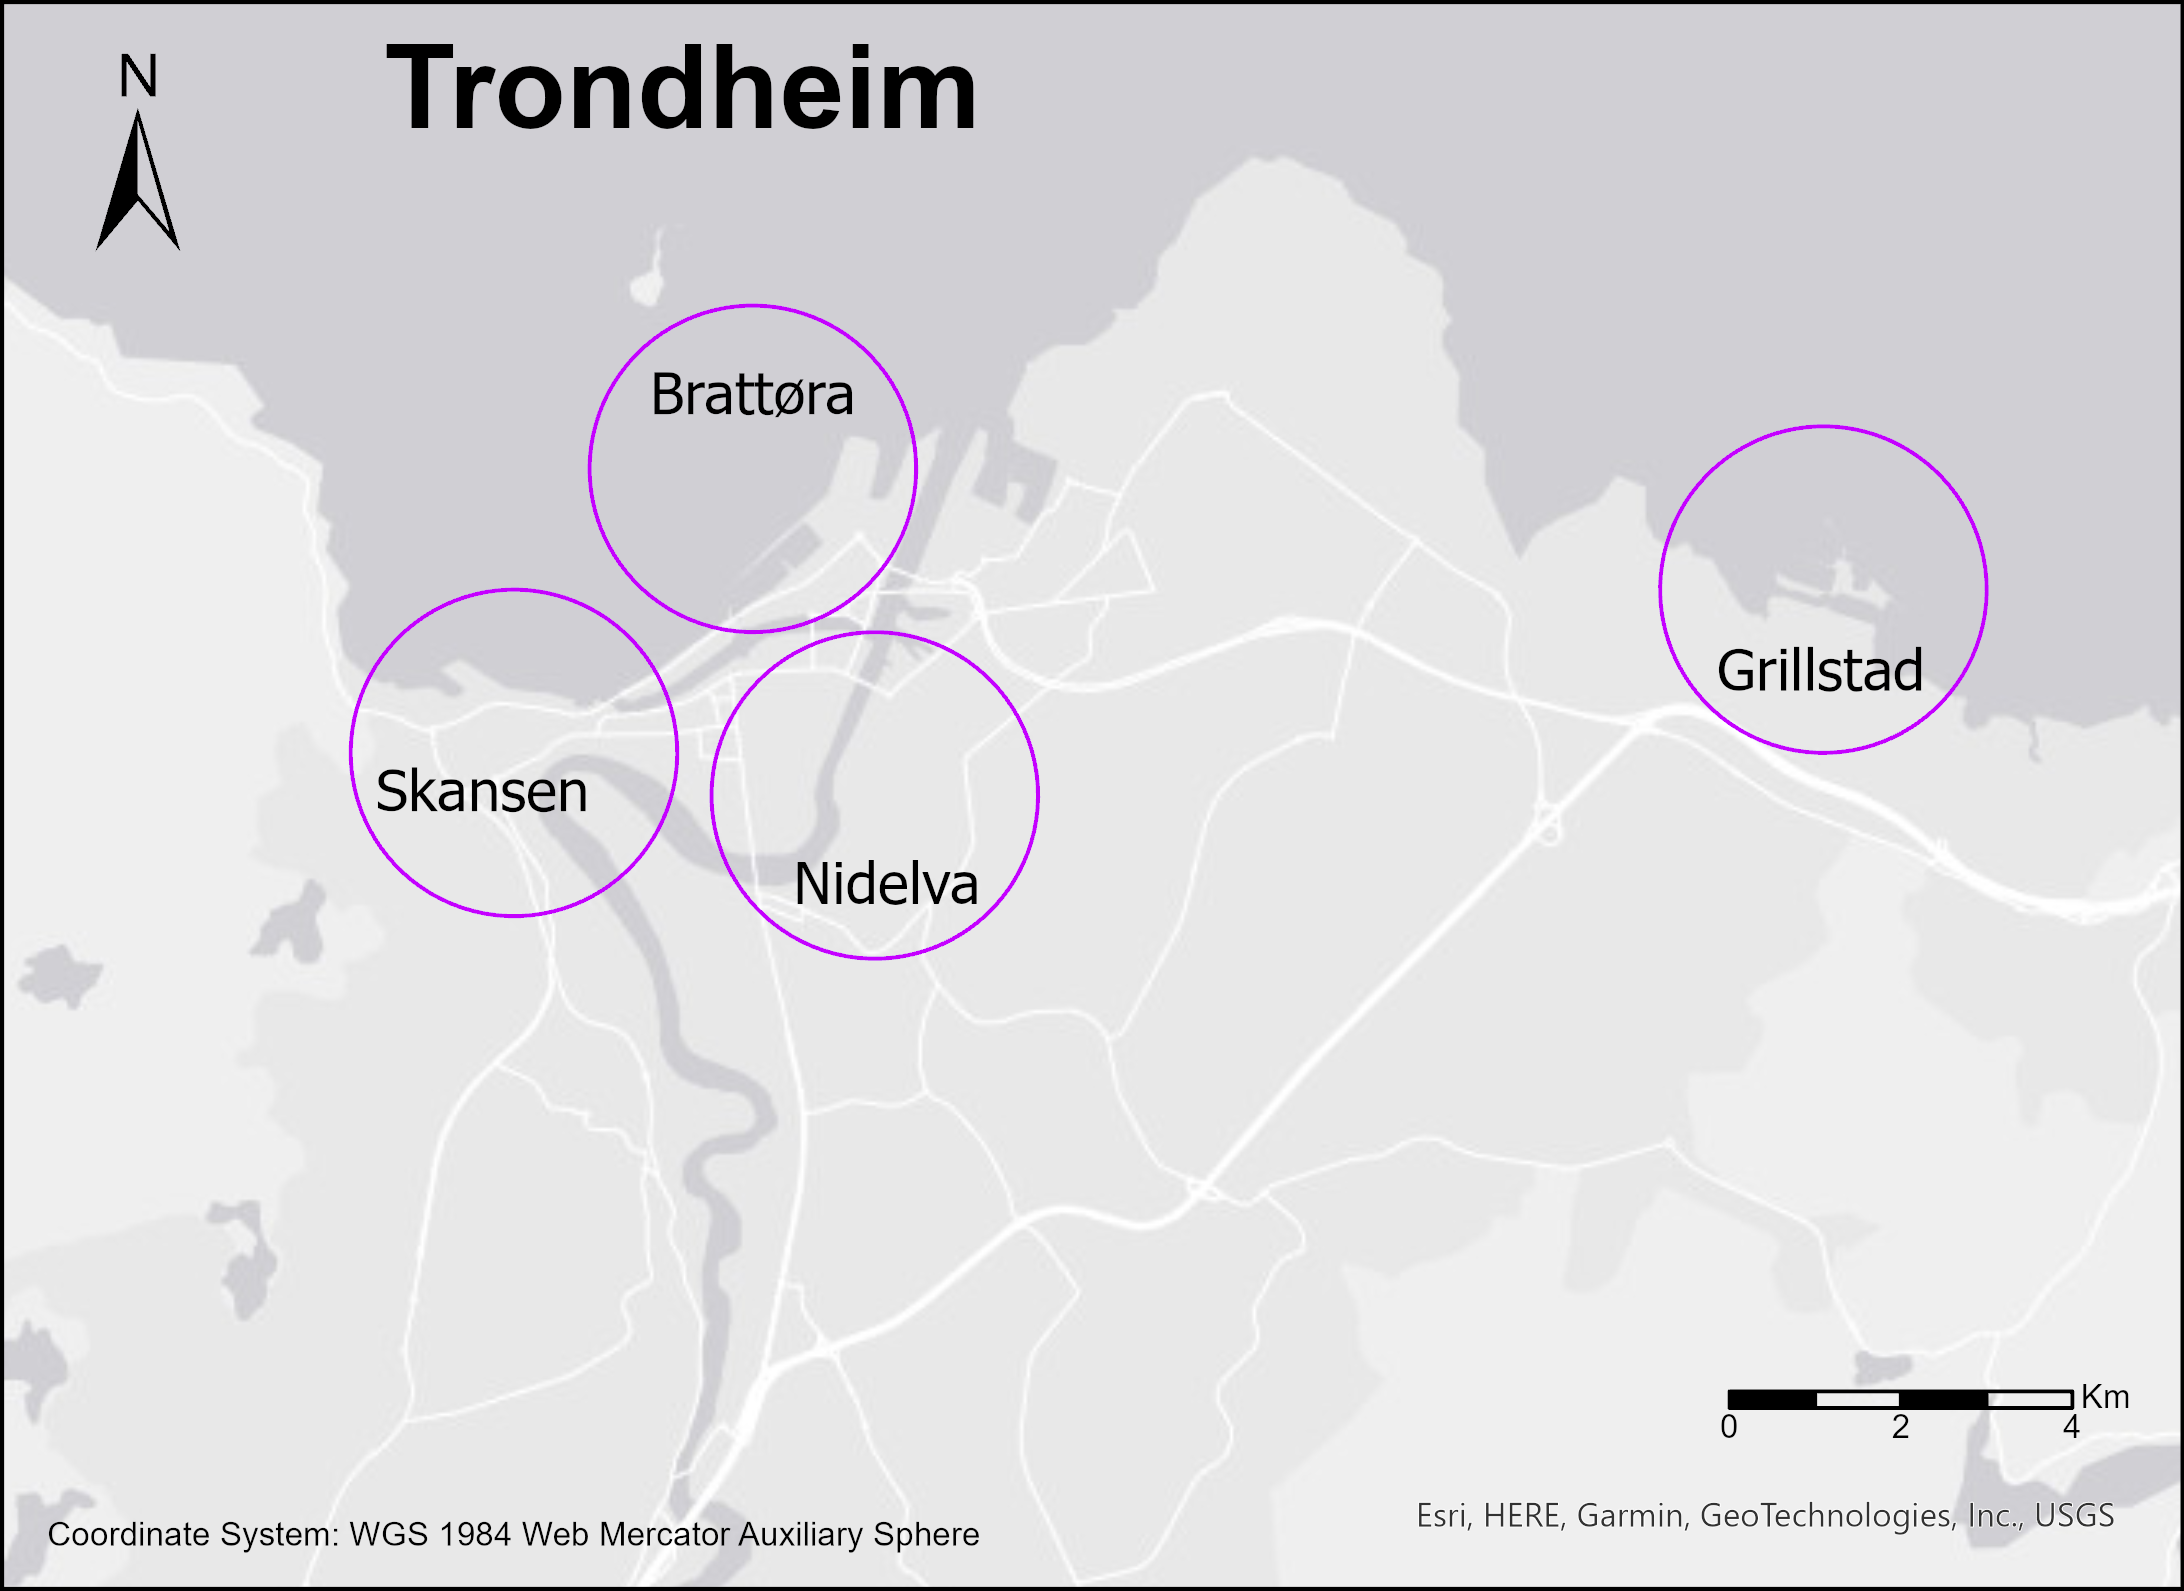
\includegraphics[width=1.0\textwidth]{fig/trondheim_research_sites_grey_circles.png}
    \caption{ The location of the Research Sites in Trondheim - The research sites are highlighted with purple circles and are called Brattøra, Grillstad, Skansen and Nidelva. Figure was created using ArcGIS Pro}
    \label{fig:research sites}
\end{figure}

\paragraph{}

Four research sites were selected based on coastal characteristics, infrastructure and high levels of daily population. Factors included in physical vulnerability are natural resistance to erosion, engineered resistance to erosion, engineered protection to sea level extremes, infrastructure directly upon coastline, settlements patterns, usage patterns and projected changes in sea level extremes. The four sites selected were Brattøra, Nidelva, Skansen and Grillstad. The physical vulnerability was determined from direct observation, kvartverket models and consulting planning documents (TEK10 /17) for each site. \cite{miljoenheten_og_byplankontoret_trondheim_kommune_9-notat-om-havnivastigning-og-stormflo---hensyn-i-arealplanlegging-nyhavnapdf_2020}


\paragraph{}
\begin{table}[!ht]
    \centering
    \begin{tabular}{|l|l|l|l|l|}
    \hline
        location & Brattøra & Grillstad & Skansen  & Nidelva \\ \hline
        PV 70 years ago & high & high & medium & Low \\ \hline
        PV now &  medium &  medium &  low &  low \\ \hline
        PV in 70 years &  high &  high &  medium &  medium \\ \hline
        Dominant & Office space  & Residential & Recreational  & Residential and \\ \newline
        use & and harbour &  only   &  and industry & and commercial  \\ \hline
        Land type & Reclaimed land & Reclaimed land & Managed coastline  & Altered tidal river \\ \hline
        protection & Harbour wall & Harbour wall & Harbour wall, placed rocks & inland \\ \hline
    \end{tabular}
    \caption{The changing physical vulnerability to sea level extremes (PV) of the Research Sites.}
    \label{table:research-sites}
\end{table}

Brattøra is the research site with the least amount of residential population. The dominant use is as office space, which is protected by a harbour wall and a small harbour behind that. The location is upon reclaimed land and for this reason it has very high physical vulnerability 70 years ago. The modern day harbour and areas design allows it to have medium physical vulnerability now, but it is projected to have several sections regularly flooded in 70 years. Currently these areas are predominantly sustainable urban development schemes with footpaths and car parks where a lot of the flooding would occur, but there is still risk of more significant impacts from sea level extremes beyond nuisance flooding, shutting off of important transport routes and preventing access to offices.
\paragraph{}
Grillstad is also located on reclaimed land and again has very high physical vulnerability 70 years ago. It is also located behind a harbour and harbour wall, in contrast to  Brattøra the dominant use is residential. There is several small commercial ventures, but the vast majority are their to serve the needs only of local residents. There is no major transport connections or industry in this sites. 
\paragraph{}
Nidelva is a less obvious choice for research into sea level extremes as it is situated further from the coastline. The land type here is altered tidal river and its physical vulnerability 70 years ago is low. The dominant use is residential and commercial and it has lower physical vulnerability predicted in 70 years than Brattøra and Grillstad. Nidelva site has the added complication of the river level potentially impacting the height of the water at certain times. The river here is controlled by the damn in.... which is part of the hydroelectric power scheme which provides energy to...
\paragraph{}
Skansen has two dominant uses of recreational and industry. However there is also significant residency in the area, the majority being high rise flats at least ***check** 100m from the coastline. While several aspects of this coastline may appear more natural it is a managed coastline which is protected by placed rocks, a harbour wall and small bays. Unlike the other sites there has been attempts to utilised natural techniques to prevent flooding in this area. This includes the restoration of Illabekken and the use of non-concreted areas which are covered in plants concrete to improve infiltration \cite{selliseth_ilabekken_2021}.
\paragraph{}

\paragraph{}
Brattøra, Skansen and Nidelva were highlighted during case presentations by the municipality as areas which can expect a risk of flooding, but that the water will then disappear again afterwards. This means they have special building requirements \cite{hanssen_saksframlegg_2013}. Grillstad was not specified in this report as it was built after, but its location is in the area requiring these special requirements so it can also be considered a biophysically vulnerable area.  


